
\section{Conclusions}\label{sec:Discussion}

This paper has made the following contributions to learning transferable models of object behaviour:

\noindent {\bf Predictors of object motion can be learned.} This is supported by experiment P1, where the behaviour of three real objects was learned by 8 of the 9 algorithm-information combinations. 

\noindent {\bf Learning transfer can be achieved.} The simulated and real runs from experiments P2 and P3 both support the hypotheses H2  and H3 that learning transfer can be achieved with respect to action and shape. The analysis of simulated runs explains why some information-algorithm combinations succeed and some do not. 

\noindent {\bf Contact information assists transfer.} We hypothesised that modelling agent-object and object-environment contacts is important for learning transferable models. This hypothesis is supported by experiments P2 and P3. In simulation adding information G+A+E can give substantial performance improvements, for both transfer to novel actions (Figure~\ref{fig:A_av_graphs}) (left panel) and to novel shapes (Figure~\ref{fig:S_av_graphs}) (bottom left).  This result held for shape transfer for one of the two real object cases. 

%\begin{table}[b]
%\begin{center}
%\begin{tabular}{|l|l|l|l|l|}
%\cline{3-5}
%\multicolumn{2}{c}{ } & \multicolumn{3}{|c|}{Information Utilised} \\
%\cline{1-5}
%Predictor & data & Global\,(G) & G\,\&\,Agent\,(A) & G\,\&\,A\,\&\,Env \\
%\cline{1-5}
%KDEF & sim & 0.189$\pm$0.004 & 0.188$\pm$0.010 & \textbf{0.025}$\pm$0.001 \\
%LWPR & sim & 0.154$\pm$0.011 & 0.083$\pm$0.007 & 0.243$\pm$0.001 \\
%KDE & sim & n/a & 0.105$\pm$0.003 & 0.315$\pm$0.001 \\
%\cline{1-5}
%KDEF & real & 0.181$\pm$0.002 & 0.134$\pm$0.003 & \textbf{0.107}$\pm$0.002 \\
%LWPR & real & 0.200$\pm$0.002 & 0.252$\pm$0.003 & 0.231$\pm$0.002 \\
%KDE & real & n/a & 0.186$\pm$0.002 & 0.198$\pm$0.001 \\
%\cline{3-5}
%PhysX & real & \multicolumn{3}{|c|}{0.103$\pm$0.003} \\
%\cline{1-5}
%\end{tabular}
%\end{center}
%\caption[Performance Table]{Experiment S-transfer: Generalisation to novel shape.
%Trained on cylinder and box, tested on double-cylinder, for simulated and real data.
%Comparative performance of predictors vs. information used.
%Shown is the dimensionless measure normalised average error ${E_{av}^{norm}} \pm$ standard error.
%}\label{tab:PerformanceTableS2av}
%\end{table}

\noindent {\bf Factorisation assists transfer.} Modelling contacts is hard. The right representation is required to exploit the available information. Experiments P2 and P3 in simulation show that factoring the density estimation problem by contacts aids learning (see Figure~\ref{fig:A_av_graphs} (left panel), and Figure~\ref{fig:S_av_graphs} (bottom left panel and top right panel). This supports the hypothesis that factorisation of information by contact assists transfer. 
\newlength{\imgCXwid}
\setlength{\imgCXwid}{2.15cm}
\begin{figure*}[tbp]
%\centerline{
%\includegraphics[width=2.3cm]{images/C1_2exp_48_1}
%\includegraphics[width=2.3cm]{images/C1_2exp_48_2}
%\includegraphics[width=2.3cm]{images/C1_2exp_48_3}
%\includegraphics[width=2.3cm]{images/C1_2exp_48_4}
%\includegraphics[width=2.3cm]{images/C1_2exp_48_5}
%}
%\vspace{0.1cm}
\centerline{
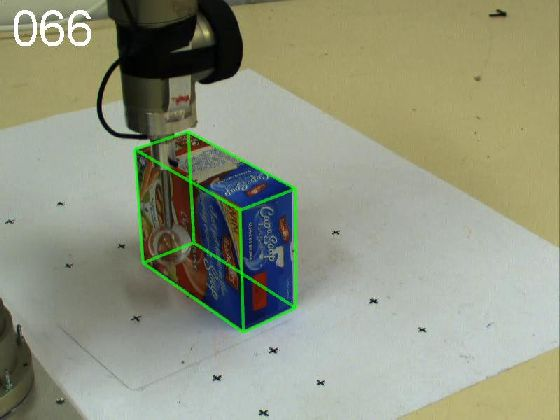
\includegraphics[width=\imgCXwid]{images/C1_2exp_87_1}
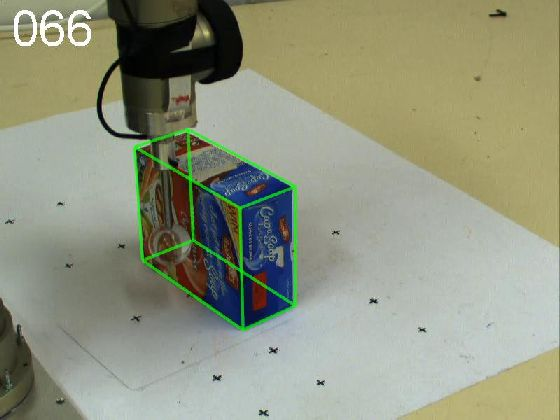
\includegraphics[width=\imgCXwid]{images/C1_1exp_87_1}
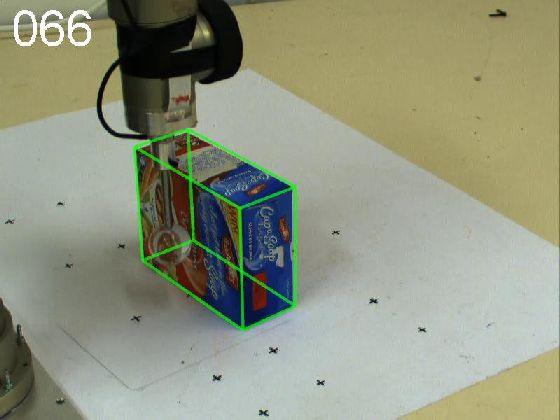
\includegraphics[width=\imgCXwid]{images/C1_LWPR1_87_1}
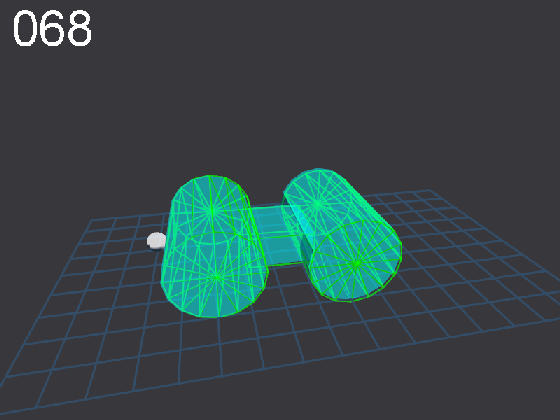
\includegraphics[width=\imgCXwid]{images/C5_1exp_6_1}
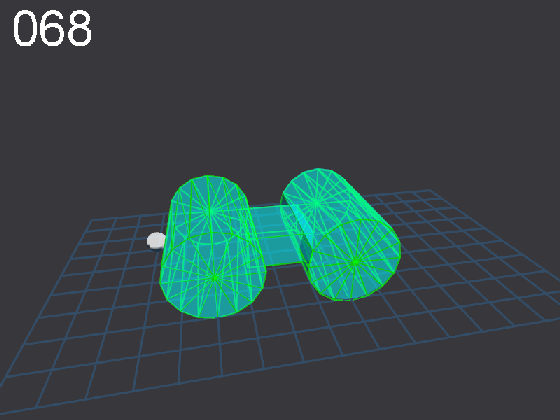
\includegraphics[width=\imgCXwid]{images/C5_2exp_6_1}
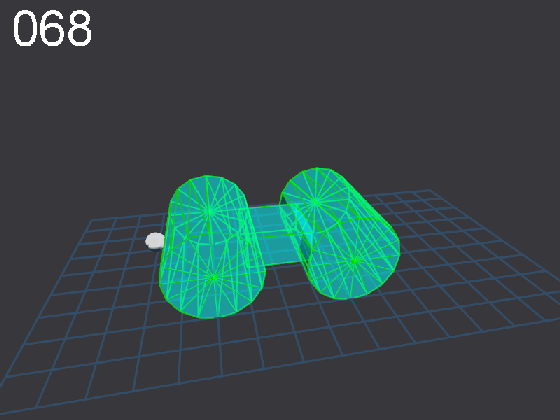
\includegraphics[width=\imgCXwid]{images/C5_3exp_6_1}
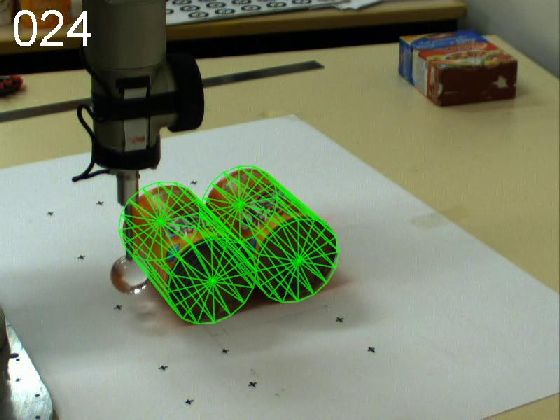
\includegraphics[width=\imgCXwid]{images/C2_3exp_75_1}
}
%\vspace{0.1cm}
\centerline{
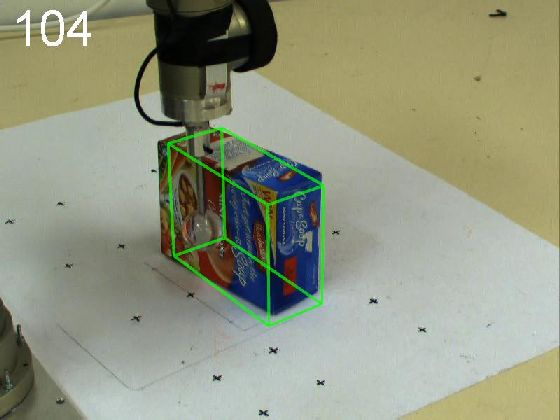
\includegraphics[width=\imgCXwid]{images/C1_2exp_87_2}
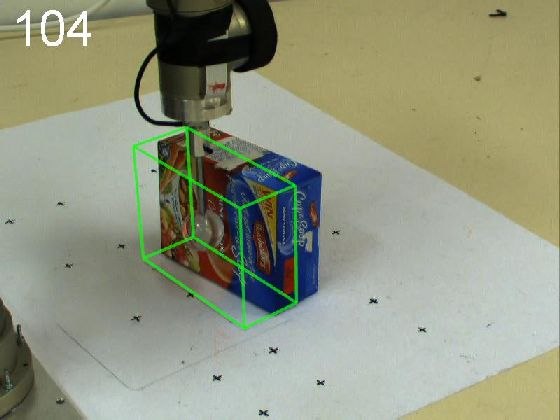
\includegraphics[width=\imgCXwid]{images/C1_1exp_87_2}
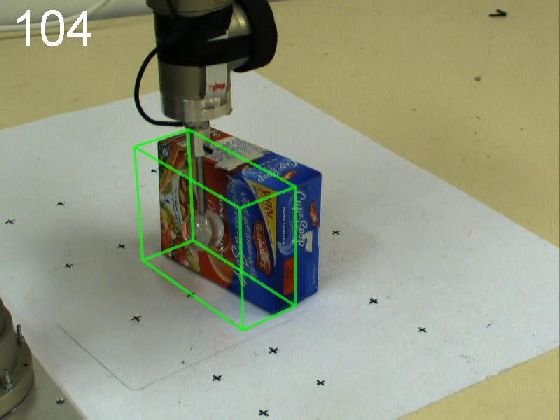
\includegraphics[width=\imgCXwid]{images/C1_LWPR1_87_2}
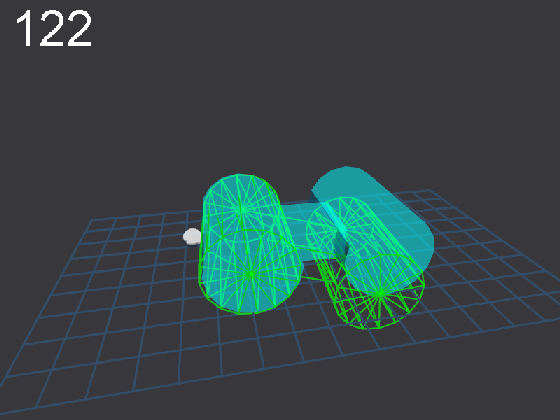
\includegraphics[width=\imgCXwid]{images/C5_1exp_6_2}
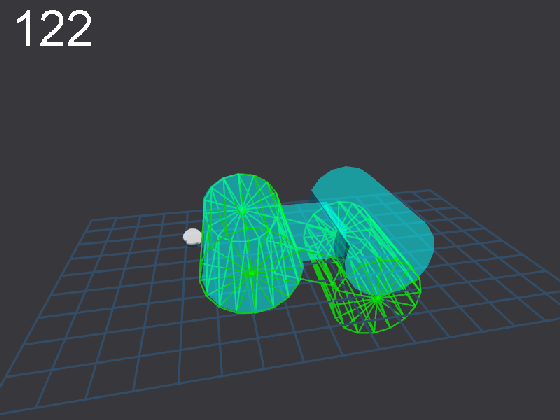
\includegraphics[width=\imgCXwid]{images/C5_2exp_6_2}
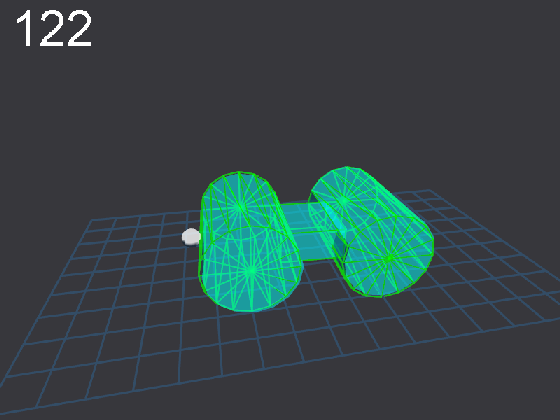
\includegraphics[width=\imgCXwid]{images/C5_3exp_6_2}
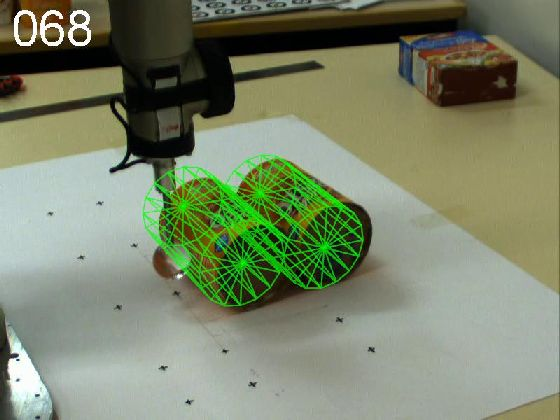
\includegraphics[width=\imgCXwid]{images/C2_3exp_75_2}
}
%\vspace{0.1cm}
\centerline{
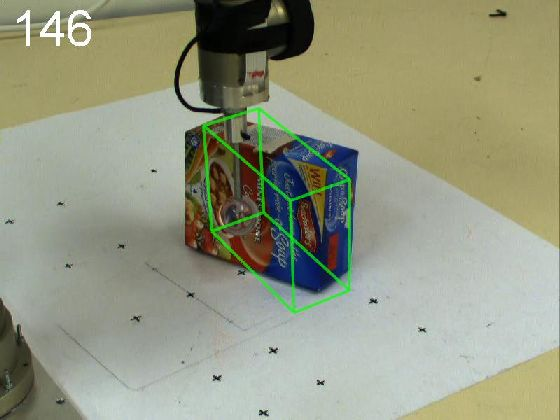
\includegraphics[width=\imgCXwid]{images/C1_2exp_87_3}
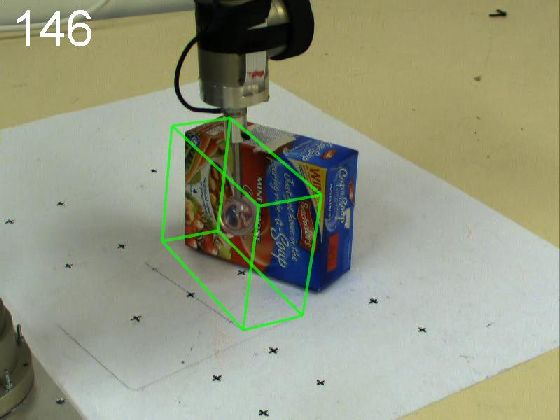
\includegraphics[width=\imgCXwid]{images/C1_1exp_87_3}
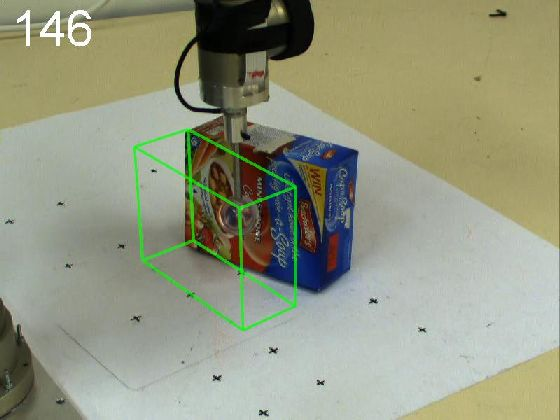
\includegraphics[width=\imgCXwid]{images/C1_LWPR1_87_3}
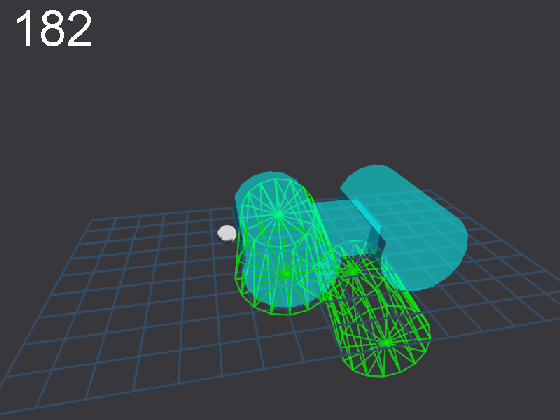
\includegraphics[width=\imgCXwid]{images/C5_1exp_6_3}
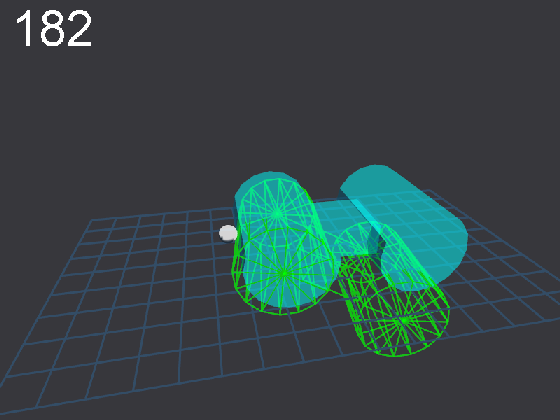
\includegraphics[width=\imgCXwid]{images/C5_2exp_6_3}
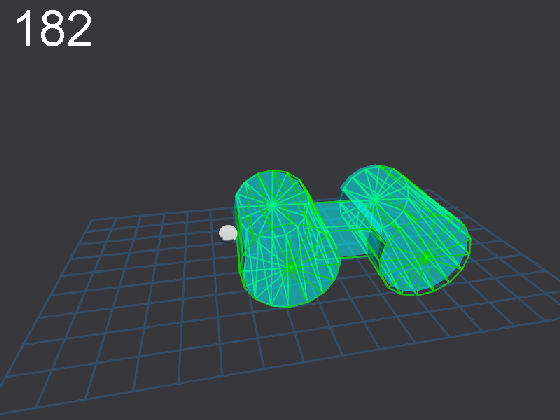
\includegraphics[width=\imgCXwid]{images/C5_3exp_6_3}
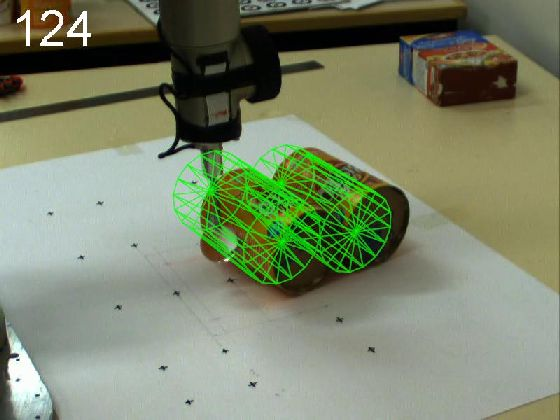
\includegraphics[width=\imgCXwid]{images/C2_3exp_75_3}
}
\centerline{
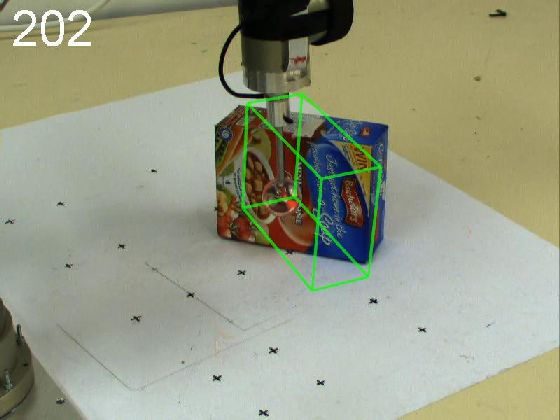
\includegraphics[width=\imgCXwid]{images/C1_2exp_87_4}
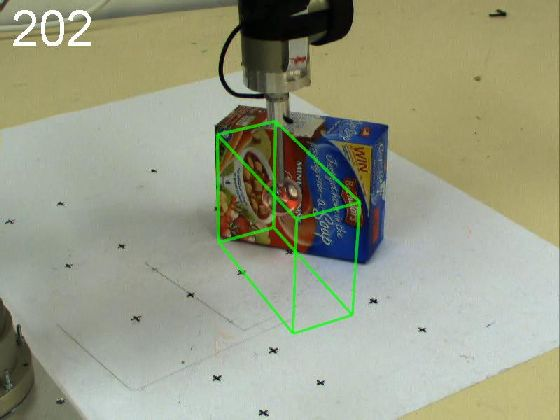
\includegraphics[width=\imgCXwid]{images/C1_1exp_87_4}
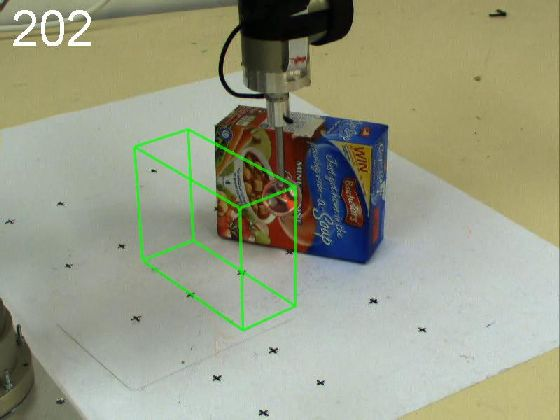
\includegraphics[width=\imgCXwid]{images/C1_LWPR1_87_4}
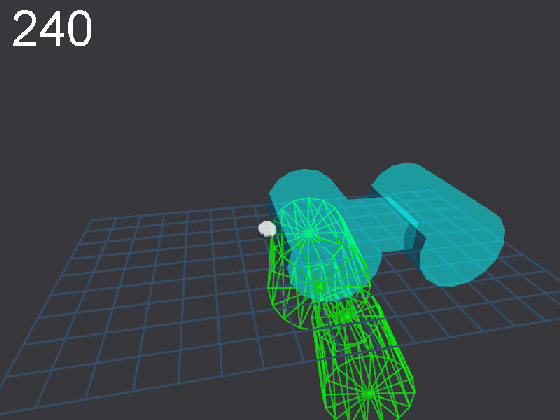
\includegraphics[width=\imgCXwid]{images/C5_1exp_6_4}
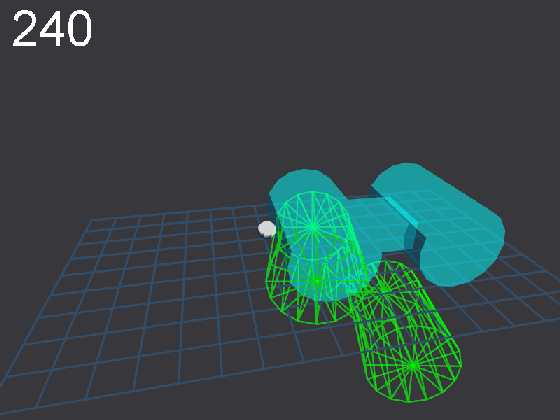
\includegraphics[width=\imgCXwid]{images/C5_2exp_6_4}
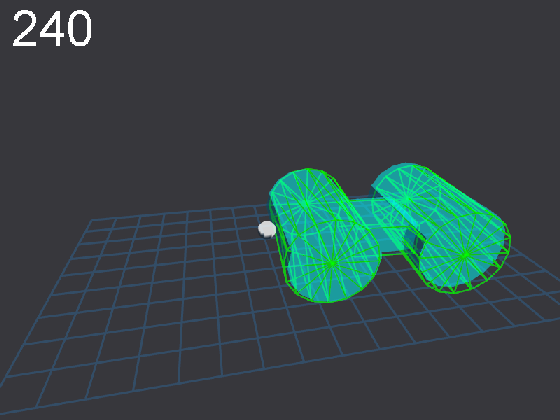
\includegraphics[width=\imgCXwid]{images/C5_3exp_6_4}
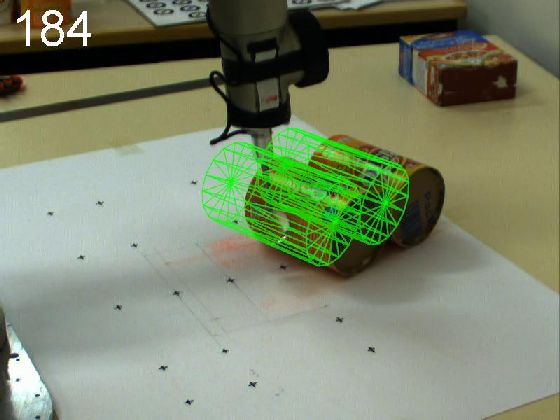
\includegraphics[width=\imgCXwid]{images/C2_3exp_75_4}
}
%\vspace{0.1cm}
\centerline{
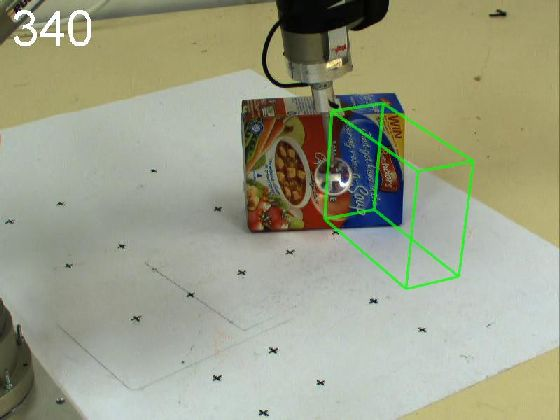
\includegraphics[width=\imgCXwid]{images/C1_2exp_87_5}
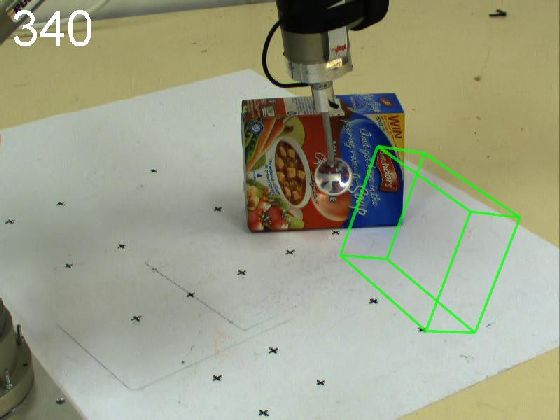
\includegraphics[width=\imgCXwid]{images/C1_1exp_87_5}
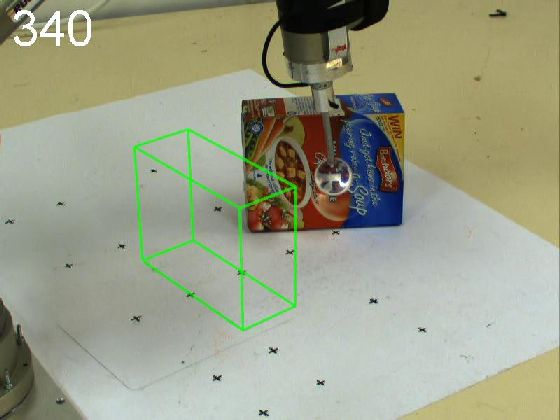
\includegraphics[width=\imgCXwid]{images/C1_LWPR1_87_5}
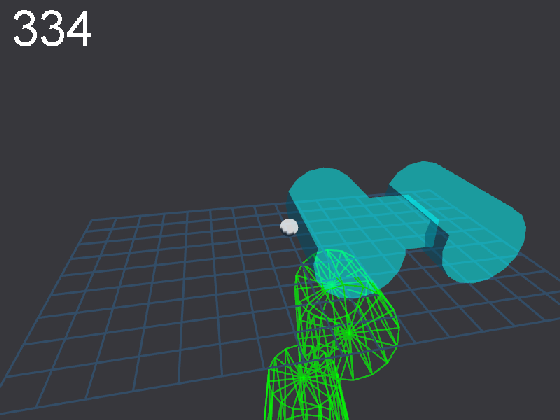
\includegraphics[width=\imgCXwid]{images/C5_1exp_6_5}
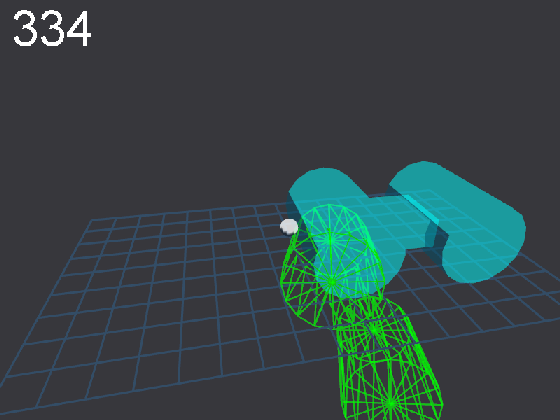
\includegraphics[width=\imgCXwid]{images/C5_2exp_6_5}
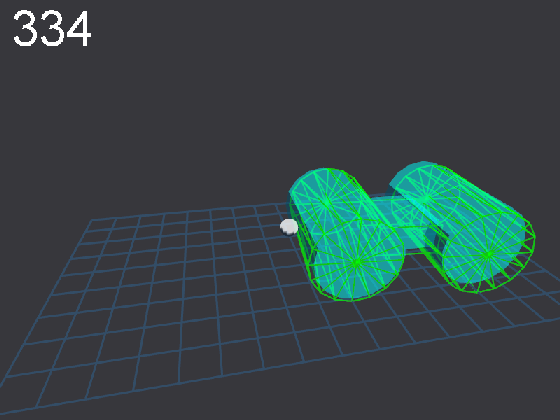
\includegraphics[width=\imgCXwid]{images/C5_3exp_6_5}
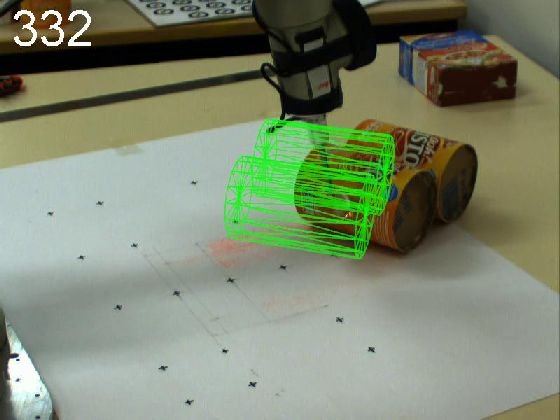
\includegraphics[width=\imgCXwid]{images/C2_3exp_75_5}
}

\caption {Experiment P3: Shape Transfer. Green outline shows predictions. Column~1: KDEF-GA/quat.
  Col~2: KDEF-G/quat. Col~3: LWPR-G for one trial.  Note that the
  KDEF-G/quat and LWPR-G methods predict that the robot finger moves
  into the box.  Col~4: KDEF-G/quat. Col~5: KDEF-GA/quat. Col~6:
  KDEF-GAE/quat. Col~7: KDEF-GAE/quat. The frame number is shown in
  the top left of each image.  }
\label{fig:ExperimentStransfer}
\end{figure*}

\noindent {\bf Learning can match or exceed physics engine performance.} In experiment P1, in 23 of 24 cases the learners significantly outperformed a tuned physics engine. The learned predictions were usually physically plausible (see Figures~\ref{fig:ExperimentL2}). This supports hypothesis H1. In experiments P2 and P3 learning transfer using factored KDE was able to match or improve on the prediction error of a physics engine (see Figures~\ref{fig:A_av_graphs} right panel and Figure~\ref{fig:S_av_graphs} top row). Its predictions were also usually physically plausible (see Figure~\ref{fig:ExperimentA} columns 4 and 7, and Figure~\ref{fig:ExperimentStransfer} columns 1,6 and 7).

\noindent {\bf Limitations and extensions:} This work is a first attempt to perform transfer learning for motion models of objects. There are two limitations to the methods presented. The most important is seen in the degradation of transfer performance in the face of observation noise. We are therefore extending our learning algorithm to take account of this noise.  The second is that at the moment learning and transfer both require selection of the attachment points of frames to each body. This process needs to be automated.


%The results presented are roughly grouped according to the three hypotheses. In the experiments L1, L2 and L3 the ability to learn from real data on a variety of objects was examined. Hypothesis 1 was that learning can outperform physics engine based prediction and is supported by Figure~\ref{fig:Setup}. In addition Tables~\ref{tab:PerformanceTableL1av}-\ref{tab:PerformanceTableL3fi} and Figures~\ref{fig:L1graphs}-\ref{fig:L3graphs} show that the quaternion encoding for the KDE approach produces a lower error in the predicted trajectories than either Euler angles or the encoding based on the von Mises-Fisher distribution; and that LWPR worsens in performance as it has more input dimensions. This is important because it shows that the regression approach, while it can learn good predictions, is not able to take advantage of additional information in the way that the product of densities approach does.
%Note that LWPR does not make use of the factorisation employed in the KDE case,
%but that instead it is given the input information that the 2 and 3 factor KDE
%learners have in order to make sure that all fair comparisons are made.
%All these experiments involved interpolative generalisation
%with respect to actions, as the actions in the test set are generated randomly from a continuous space,
%and thus differ from those in the training set while being drawn from the same distribution.

%Experiment A tested Hypothesis 2 -- that learning can generalise extrapolatively to novel actions.
%Tables~\ref{tab:PerformanceTableAav} and \ref{tab:PerformanceTableAfi} show that
%this is the case for 2 and 3 factor versions of the KDE approach,
%but not for a single global factor for either KDE or for any of the treatments using LWPR.
%This shows that the hypothesis is correct,
%and supports our intuition as to why having a product of factors will help
%(Figure~\ref{fig:ToyExample}). This is shown particularly clearly by
%Figures~\ref{fig:ExperimentAsim} and \ref{fig:ExperimentAreal}.

%Experiments S1, S2 and S3 tested Hypothesis 3 -- that learning can generalise interpolatively and extrapolatively to novel shapes. Tables~\ref{tab:PerformanceTableS1av} to \ref{tab:PerformanceTableS3fi} show that errors are larger for extrapolative generalisation than interpolative generalisation. The Tables suggest, for both simulated and real data, that KDE outperforms LWPR (although note the one exception to this in Table~\ref{tab:PerformanceTableS1fi}). Illustrative cases are shown in Figures~\ref{fig:ExperimentS1} to \ref{fig:ExperimentS3}.

%Finally it is important that the predictions are what a viewer would judge as qualitatively good, ie. that the direction of travel, and the qualitative motions of the objects are correct. This is supported for Experiments L1-3 by Figures~\ref{fig:ExperimentL1} to \ref{fig:ExperimentL3}, where it can be seen that the paths followed by the predictions and the objects match, even when the precise timing of the trajectories sometimes differs. %check that Fig exptL3 really shows rolling. 
%In Figures~\ref{fig:ExperimentAsim} to \ref{fig:ExperimentS2real} it can be seen that predictions on simulated data are more accurate that those on real data, but that although divergence occurs between the predictions and the real data the predictions produced still show the correct direction of travel, and are physically plausible except for a degree of object-finger interpenetration in Figure~\ref{fig:ExperimentS2real}. It is worth noting that only the KDE learners produced plausible predictions for shape generalisation and action generalisation. In every case for experiments A and S1, the regression prediction was that the object failed to move, with the finger passing straight through the object.

This paper establishes that predictions of object behaviour can be learned using a variety of techniques; that they can outperform physics engine predictions; that they can generalise interpolatively to similar actions and shapes; that they can be transfered to novel actions and shapes, and that they produce physically plausible predictions. Transfer learning of such models, while challenging, is possible with the right representation.  In particular a factored problem formulation encodes transferable predictions that are physically plausible and qualitatively correct.